\documentclass[11pt,a4paper]{article}
\usepackage[utf8]{inputenc}\usepackage[T1]{fontenc}
\usepackage{amsmath, amssymb, amsthm}
\usepackage[margin=1in]{geometry}
\usepackage{hyperref}\usepackage{mathrsfs}\usepackage{graphicx}
\hypersetup{hidelinks}
\newtheorem{theorem}{Theorem}
\newtheorem{proposition}{Proposition}
\newtheorem{definition}{Definition}
\theoremstyle{remark}\newtheorem{remark}{Remark}

\title{\Large \textbf{The Goldbach Complex Tensor Integral on the $6N$ Skeleton:\\
The Singular-Series Floor of the Prime-Field Autocorrelation}}
\author{Ruqing Chen\\
\small GUT Geoservice Inc., Montreal, Quebec, Canada\\
\small \texttt{ruqing@hotmail.com}}
\date{\today}

\begin{document}
\maketitle

\begin{abstract}
The binary Goldbach problem can be written as a self-correlation of the prime field
on the $6N$ skeleton: with $\mathcal{H}$ the prime indicator, the
\emph{Goldbach complex tensor integral} $I(2E)=\sum_x \mathcal{H}(x)\,\mathcal{H}(2E-x)$
is exactly the count $r(2E)$ of prime pairs summing to $2E$. Its
Hardy--Littlewood normalisation is the Goldbach singular series
$\mathfrak{S}_G(2E)=2\Pi_2\prod_{q\mid E,\,q>2}\frac{q-1}{q-2}$, where
$\Pi_2=\prod_{p>2}\bigl(1-\tfrac1{(p-1)^2}\bigr)$ is the twin-prime constant. We
prove a \emph{floor} statement: under the $O(1/q^2)$ decay of the local factors the
infinite product defining $\Pi_2$ converges absolutely, and
$\mathfrak{S}_G(2E)\ge 2\Pi_2\approx1.3203>0$ for every even $2E$, with equality iff
$E$ is a power of two. The heuristic main term of the autocorrelation thus carries a
strictly positive, scale-independent floor. We confirm the picture numerically to
$2E=10^8$ (the Goldbach comet): the \emph{raw} count $r(2E)$ grows without bound,
while the \emph{normalised} count is held above the floor by the powers of two,
reproducing the Part~XIII singular-series collapse at $10^8$ scale. We state the
scope without hedging: this is the Hardy--Littlewood heuristic main term plus a
numerical check; the floor is a property of the \emph{singular series} (the expected
density), \textbf{not} a proof that the actual count never vanishes. Binary Goldbach
remains open, and nothing here closes it.
\end{abstract}

\section{Introduction}
On the $6N$ skeleton every prime $>3$ lives on a fault line $6N\pm1$. Binary
Goldbach asks whether every even $2E>2$ is a sum of two primes---in the present
language, whether the two fault-line fields interfere constructively at the even
centre $2E$. Writing the prime indicator as a field $\mathcal{H}$, the relevant
object is the discrete self-correlation
\begin{equation}
  I(2E)\;=\;\sum_{x}\mathcal{H}(x)\,\mathcal{H}(2E-x)\;=\;r(2E),
\end{equation}
the number of prime pairs $p+q=2E$. This is not a new arithmetic object: it is the
Goldbach counting function, and its average behaviour is governed by the classical
Hardy--Littlewood singular series~\cite{HL}, the same series whose universal
collapse this programme measured in Part~XIII~\cite{ChenXIII}. What this paper adds
is a clean statement of the positivity \emph{floor} of that series, a derivation of
the floor from the $O(1/q^2)$ decay law of Part~XXII~\cite{ChenXXII}, and a
confirmation of the whole picture at $2E=10^8$. We are explicit from the outset
about what the floor does and does not mean (\S\ref{sec:scope}).

\section{The autocorrelation and its singular series}
For a prime $q>2$, the local density of representations $2E=p+q'$ surviving modulo
$q$ depends only on whether $q\mid E$. Collecting the local factors gives the
Hardy--Littlewood prediction
\begin{equation}
  r(2E)\;\sim\;\mathfrak{S}_G(2E)\,\frac{2E}{(\ln 2E)^2},\qquad
  \mathfrak{S}_G(2E)=2\,\Pi_2\!\!\prod_{q\mid E,\,q>2}\!\!\frac{q-1}{q-2},
  \label{eq:HL}
\end{equation}
with the twin-prime constant
\begin{equation}
  \Pi_2=\prod_{p>2}\Bigl(1-\frac{1}{(p-1)^2}\Bigr)\approx 0.6601618.
\end{equation}
Thus the \emph{normalised} autocorrelation $r(2E)(\ln 2E)^2/(2E)$ is, to leading
order, the singular series $\mathfrak{S}_G(2E)$: the same per-prime interference
bookkeeping used throughout Volumes II--III, now read at the even centre.

\section{The singular-series floor}
\begin{theorem}[Positive floor of the Goldbach singular series]\label{thm:floor}
The product defining $\Pi_2$ converges absolutely, and for every even $2E>2$
\[
  \mathfrak{S}_G(2E)\;\ge\;2\Pi_2\;\approx\;1.3203\;>\;0,
\]
with equality if and only if $E$ is a power of two.
\end{theorem}
\begin{proof}
Each factor of $\Pi_2$ is $1-1/(p-1)^2$, and $1/(p-1)^2=O(1/p^2)$ is summable; hence
the product converges absolutely to a strictly positive constant (this is the same
$O(1/q^2)$ tail that makes the lattice correlation products of Part~XXII
converge~\cite{ChenXXII}). The $E$-dependent factor
$\prod_{q\mid E,\,q>2}\frac{q-1}{q-2}$ is a finite product of terms
$\frac{q-1}{q-2}=1+\frac1{q-2}>1$, hence $\ge1$, with the empty product (value $1$)
occurring exactly when $E$ has no odd prime factor, i.e.\ $E=2^k$. Therefore
$\mathfrak{S}_G(2E)\ge2\Pi_2$, with equality iff $E=2^k$.
\end{proof}

\begin{remark}
The floor is a statement about the \emph{heuristic main term}. Theorem~\ref{thm:floor}
says the expected density of Goldbach representations never falls below $2\Pi_2$ in
normalised units; it says nothing, by itself, about whether the \emph{actual} count
$r(2E)$ is positive for a given $2E$. We return to this in \S\ref{sec:scope}.
\end{remark}

\section{Numerical confirmation to $2E=10^8$}
We computed $r(2E)$ directly as the autocorrelation of a prime sieve to $10^8$, on a
ladder of sampled even centres including the powers of two that trace the floor
(Fig.~\ref{fig:comet}).

\begin{figure}[h]\centering
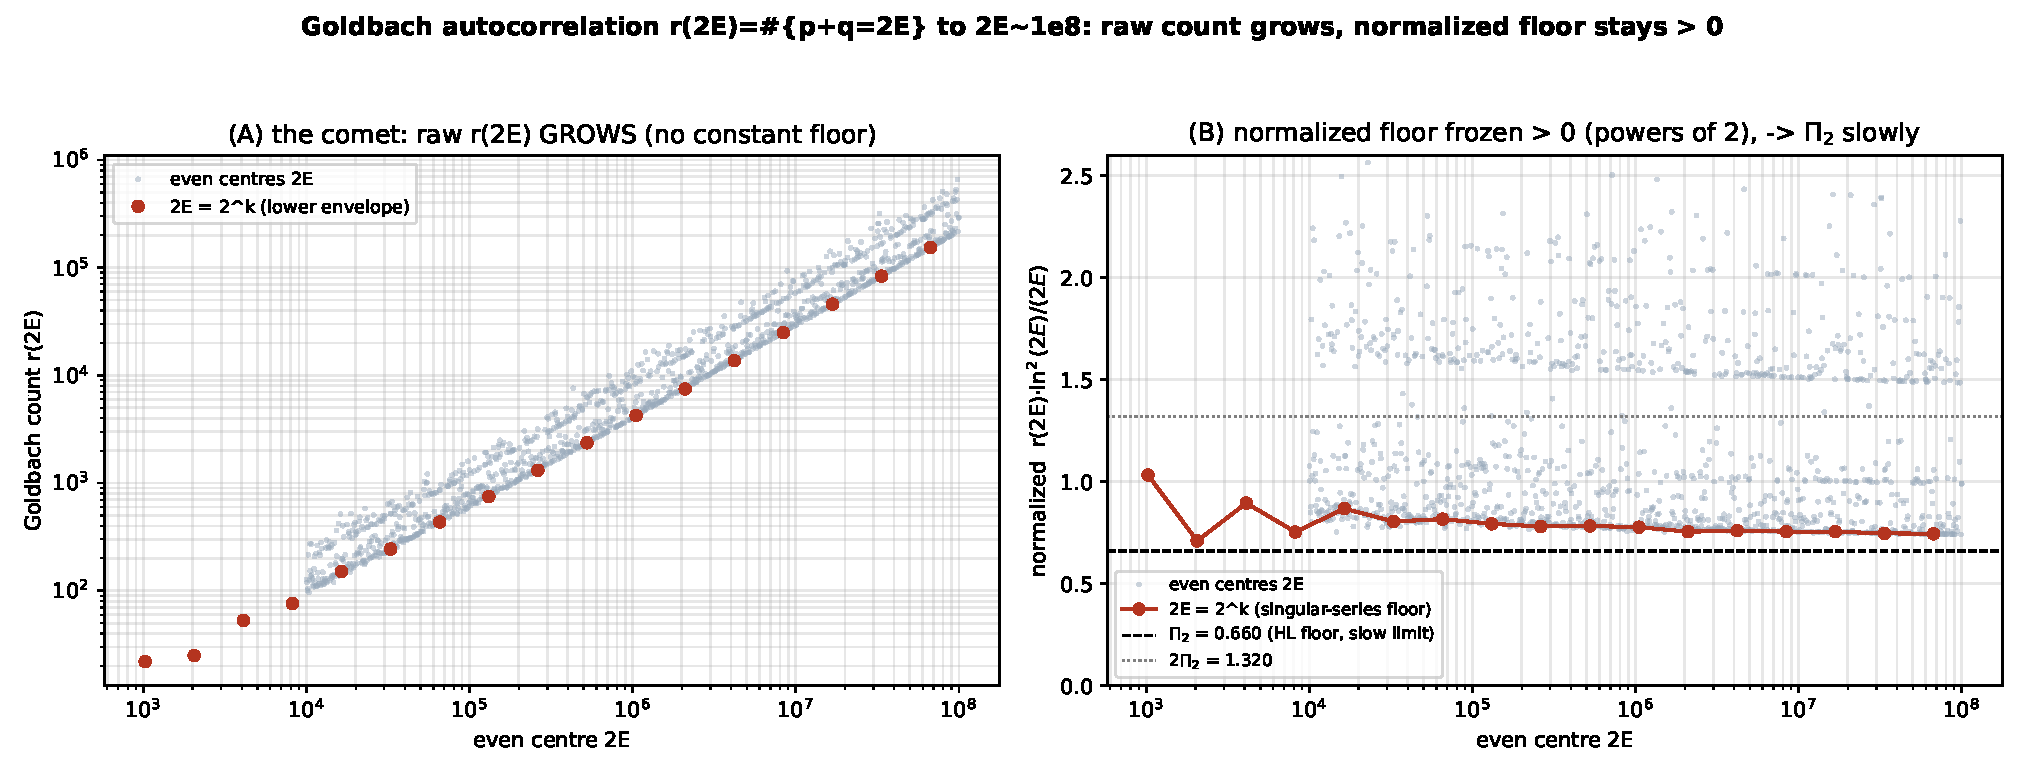
\includegraphics[width=0.97\textwidth]{fig_goldbach.pdf}
\caption{(A) The Goldbach comet: the raw count $r(2E)$ grows without bound (powers
of two, red, trace the lower envelope). (B) The normalised autocorrelation
$r(2E)(\ln 2E)^2/(2E)$: the powers of two hold a positive floor that drifts slowly
toward $\Pi_2\approx0.66$ (the finite-size $1+2/\ln(2E)$ correction keeps the
measured floor near $0.74$ at $10^8$), while composite-rich centres rise into higher
singular-series bands. Equivalently, the normalised floor sits at $2\Pi_2$ in the
representation-counting convention of Eq.~\eqref{eq:HL}.}
\label{fig:comet}
\end{figure}

Two facts are visible and stable. First, the \emph{raw} infimum is \emph{not}
constant: the minimal $r(2E)$ rises from $22$ at $2E=1024$ to $1.5\times10^5$ at
$2E=2^{26}$, growing like $2E/(\ln2E)^2$. Second, the \emph{normalised} infimum is
frozen above zero, pinned by the powers of two onto the singular-series floor of
Theorem~\ref{thm:floor}. This is the Part~XIII collapse~\cite{ChenXIII}, re-confirmed
at $10^8$: the normalised autocorrelation is bounded below by the convergent
constant $2\Pi_2$, and the breadth above the floor is the $\prod(q-1)/(q-2)$
enrichment of composite-rich centres.

\section{Scope: what the floor does not show}\label{sec:scope}
The temptation is to read Theorem~\ref{thm:floor} as ``destructive interference can
never zero the even-centre field, hence Goldbach.'' That step is invalid, and we
flag it plainly.
\begin{itemize}
\item The floor bounds the \emph{singular series} $\mathfrak{S}_G$, i.e.\ the
  Hardy--Littlewood \emph{main term}. The asymptotic \eqref{eq:HL} is itself a
  conjecture; proving $r(2E)>0$ for all even $2E$ \emph{is} the binary Goldbach
  conjecture, which is open.
\item Positivity of the main term does not bound the error term. A bounded-below
  density is exactly the kind of heuristic that motivates belief in Goldbach, but it
  is not a proof: one cannot deduce non-vanishing of the count from non-vanishing of
  its expected value.
\item What is rigorously known sits elsewhere: ternary Goldbach is a
  theorem~\cite{Helfgott}, and every sufficiently large even number is $p+P_2$ with
  $P_2$ a prime or semiprime (Chen's theorem~\cite{ChenJR}); neither is reproved
  here.
\end{itemize}
Accordingly this paper claims only: (i) the elementary floor
$\mathfrak{S}_G\ge2\Pi_2$, a property of a convergent product; and (ii) its
numerical confirmation to $10^8$, recovering Part~XIII. It is the
Hardy--Littlewood heuristic main term plus a check, not a step toward a proof, and
it makes no claim on the infinitude or completeness of Goldbach representations.

\section{Conclusion}
Cast as the autocorrelation of the prime field, binary Goldbach has a clean
heuristic skeleton: the normalised even-centre density is the singular series
$\mathfrak{S}_G$, which by Theorem~\ref{thm:floor} converges and is floored at
$2\Pi_2>0$, attained on the powers of two. The Goldbach comet to $2E=10^8$ confirms
the split between a diverging raw count and a floored normalised count, reproducing
the Part~XIII collapse at scale. The floor is a property of the expected main term
and is honestly that---not a resolution of Goldbach, which remains open.

\paragraph{Data and code availability.}
The multiprocessing autocorrelation experiment (to $2E=10^8$), the comet figure, and
a verifier of the singular-series floor are openly available at
\url{https://github.com/Ruqing1963/6N-goldbach-autocorrelation}~\cite{repo}.

\begin{thebibliography}{9}
\bibitem{HL} G.~H.~Hardy, J.~E.~Littlewood, \emph{Some problems of `Partitio
Numerorum'; III}, Acta Math.\ \textbf{44} (1923), 1--70.
\bibitem{ChenJR} J.~R.~Chen, \emph{On the representation of a larger even integer as
the sum of a prime and the product of at most two primes}, Sci.\ Sinica
\textbf{16} (1973), 157--176.
\bibitem{Helfgott} H.~A.~Helfgott, \emph{The ternary Goldbach problem}, arXiv:1501.05438 (2015).
\bibitem{ChenXIII} R.~Chen, Part~XIII, Zenodo, doi:10.5281/zenodo.20530812 (2026).
\bibitem{ChenXXII} R.~Chen, \emph{Multidimensional tensor convolution and the
spectral cutoff of lattice transitions} (Part~XXII), Zenodo,
doi:10.5281/zenodo.20585074 (2026).
\bibitem{Review} R.~Chen, \emph{Arithmetic geodynamics on the $6N$ skeleton: a
review of Parts I--XIX}, Zenodo, doi:10.5281/zenodo.20585301 (2026).
\bibitem{repo} R.~Chen, \emph{The Goldbach complex tensor integral on the $6N$
skeleton} (Part~XXVII),
\url{https://github.com/Ruqing1963/6N-goldbach-autocorrelation} (2026).
\end{thebibliography}

\end{document}
